\subsection{Status}

\begin{frame}{Status}
\begin{block}{Last milestone}
\begin{itemize}
	\item[\textcolor{black}{\VarClock}] Surface reconstruction with the VTK Toolbox

\end{itemize}
\end{block}
\begin{block}{Today}
\begin{itemize}
	\item[\textcolor{green}{\Checkmark}] Extraction of voxel data from Topy
	\item[\textcolor{green}{\Checkmark}] 3D Dual Contouring program 
	\item[\textcolor{green}{\Checkmark}] Coarsening and non-manifold edge treatment 
	\item[\textcolor{green}{\Checkmark}] Projection to quads and respective parametrization
	\item[\textcolor{black}{\VarClock}]  Interface to NURBs
\end{itemize}
\end{block}
\end{frame}






\subsection{Dual Contouring}

\begin{frame}

	\frametitle{From Voxel to Mesh Geometry}
	
	\begin{itemize}
	\item Extract isosurface from voxel information
	\item Algorithms: Marching Cubes, Dual Contouring, Extended Models
	\item Problems with VTK's Marching Cube implementation
	\end{itemize}
	\begin{figure}
	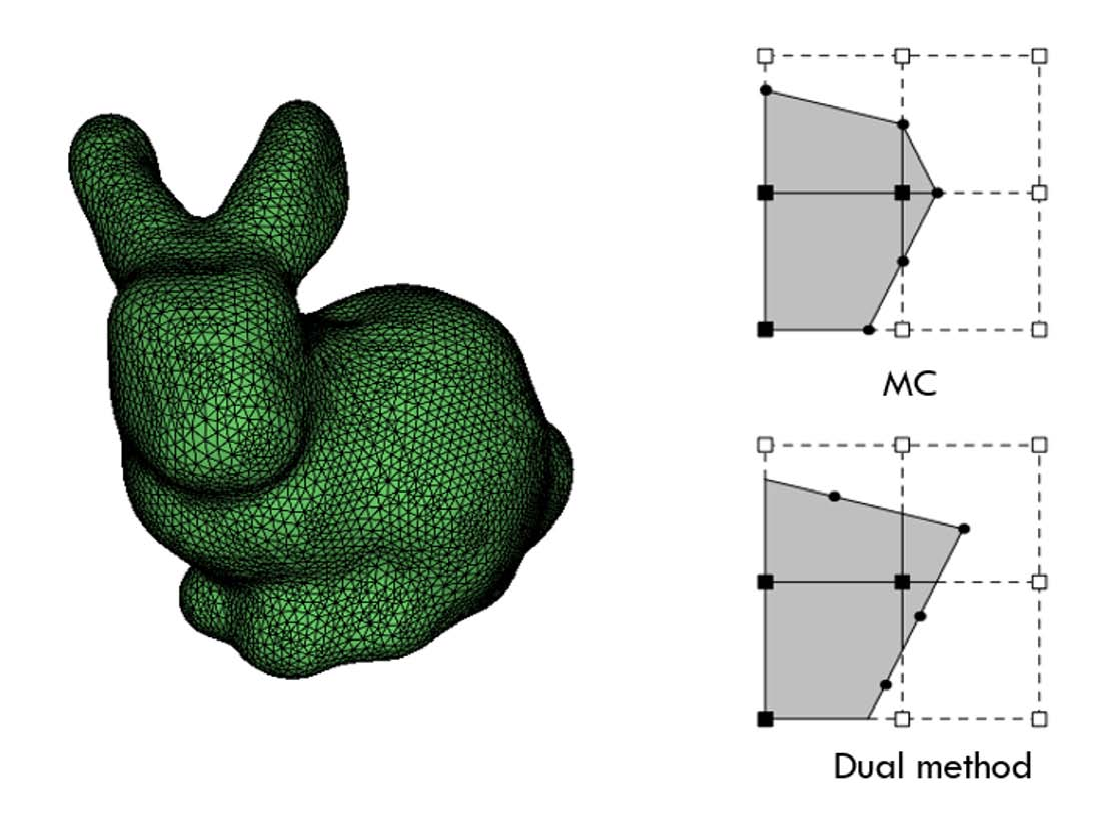
\includegraphics[scale=0.35]{Pictures/bunny_MC.pdf}
	\end{figure}
	
\end{frame}

\begin{frame}

	\frametitle{Dual Contouring}
	
	\begin{itemize}
	\item Python implementation- Use of powerful libraries, including VTK
	\item Output: Closed surface made out of \textit{quads}
	\item Coarsening is needed for surface fitting's algorithms
	\end{itemize}
	\begin{figure}
	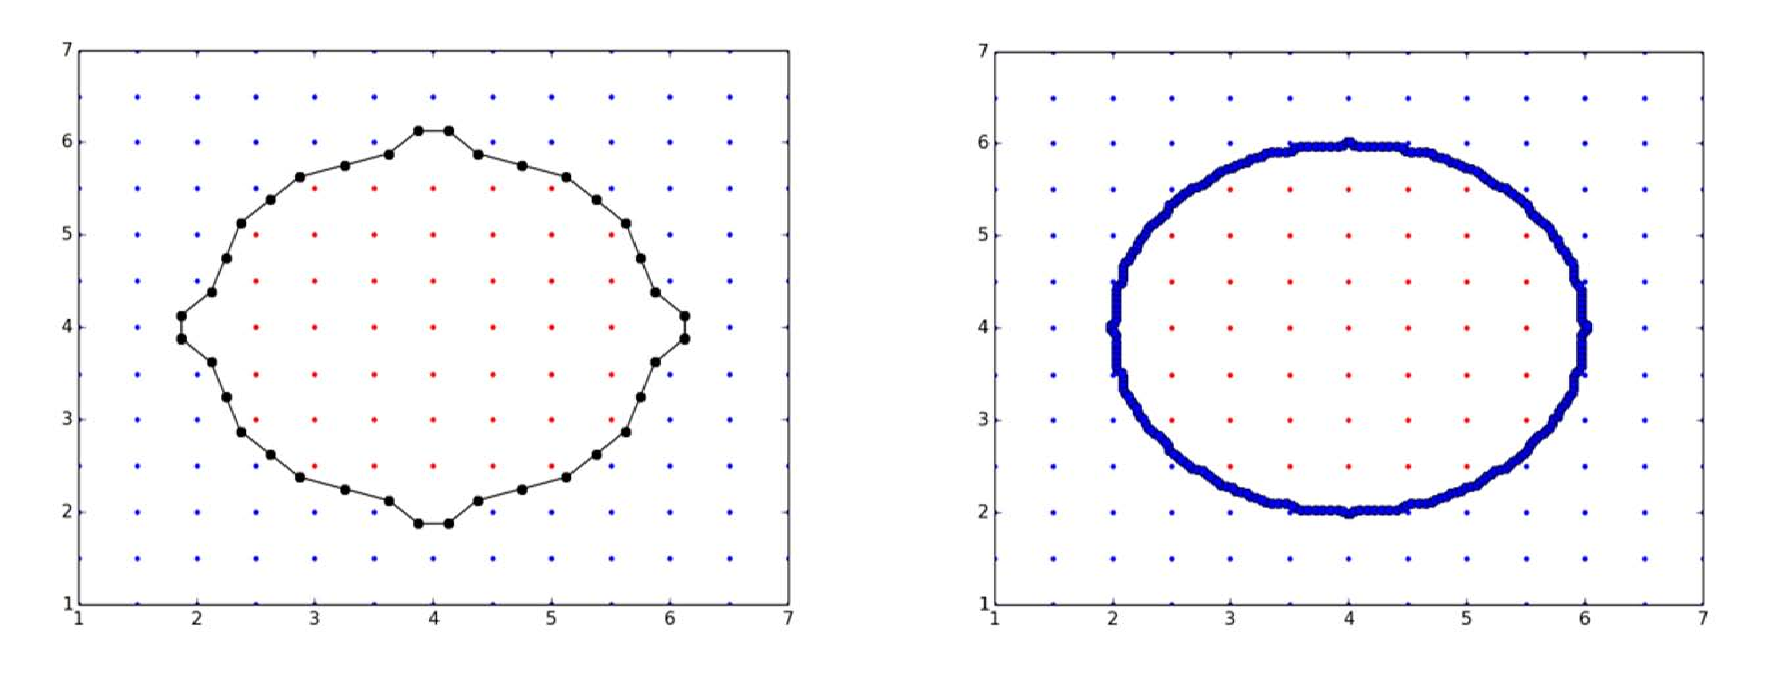
\includegraphics[scale=0.35]{Pictures/DC/DC_1.pdf}
	\end{figure}
	
\end{frame}

\begin{frame}

	\frametitle{Dual Contouring}
	
	\begin{itemize}
	\item Python implementation- Use of powerful libraries, including VTK
	\item Output: Closed surface made out of \textit{quads}
	\item Coarsening is needed for surface fitting's algorithms
	\end{itemize}
	\begin{figure}
	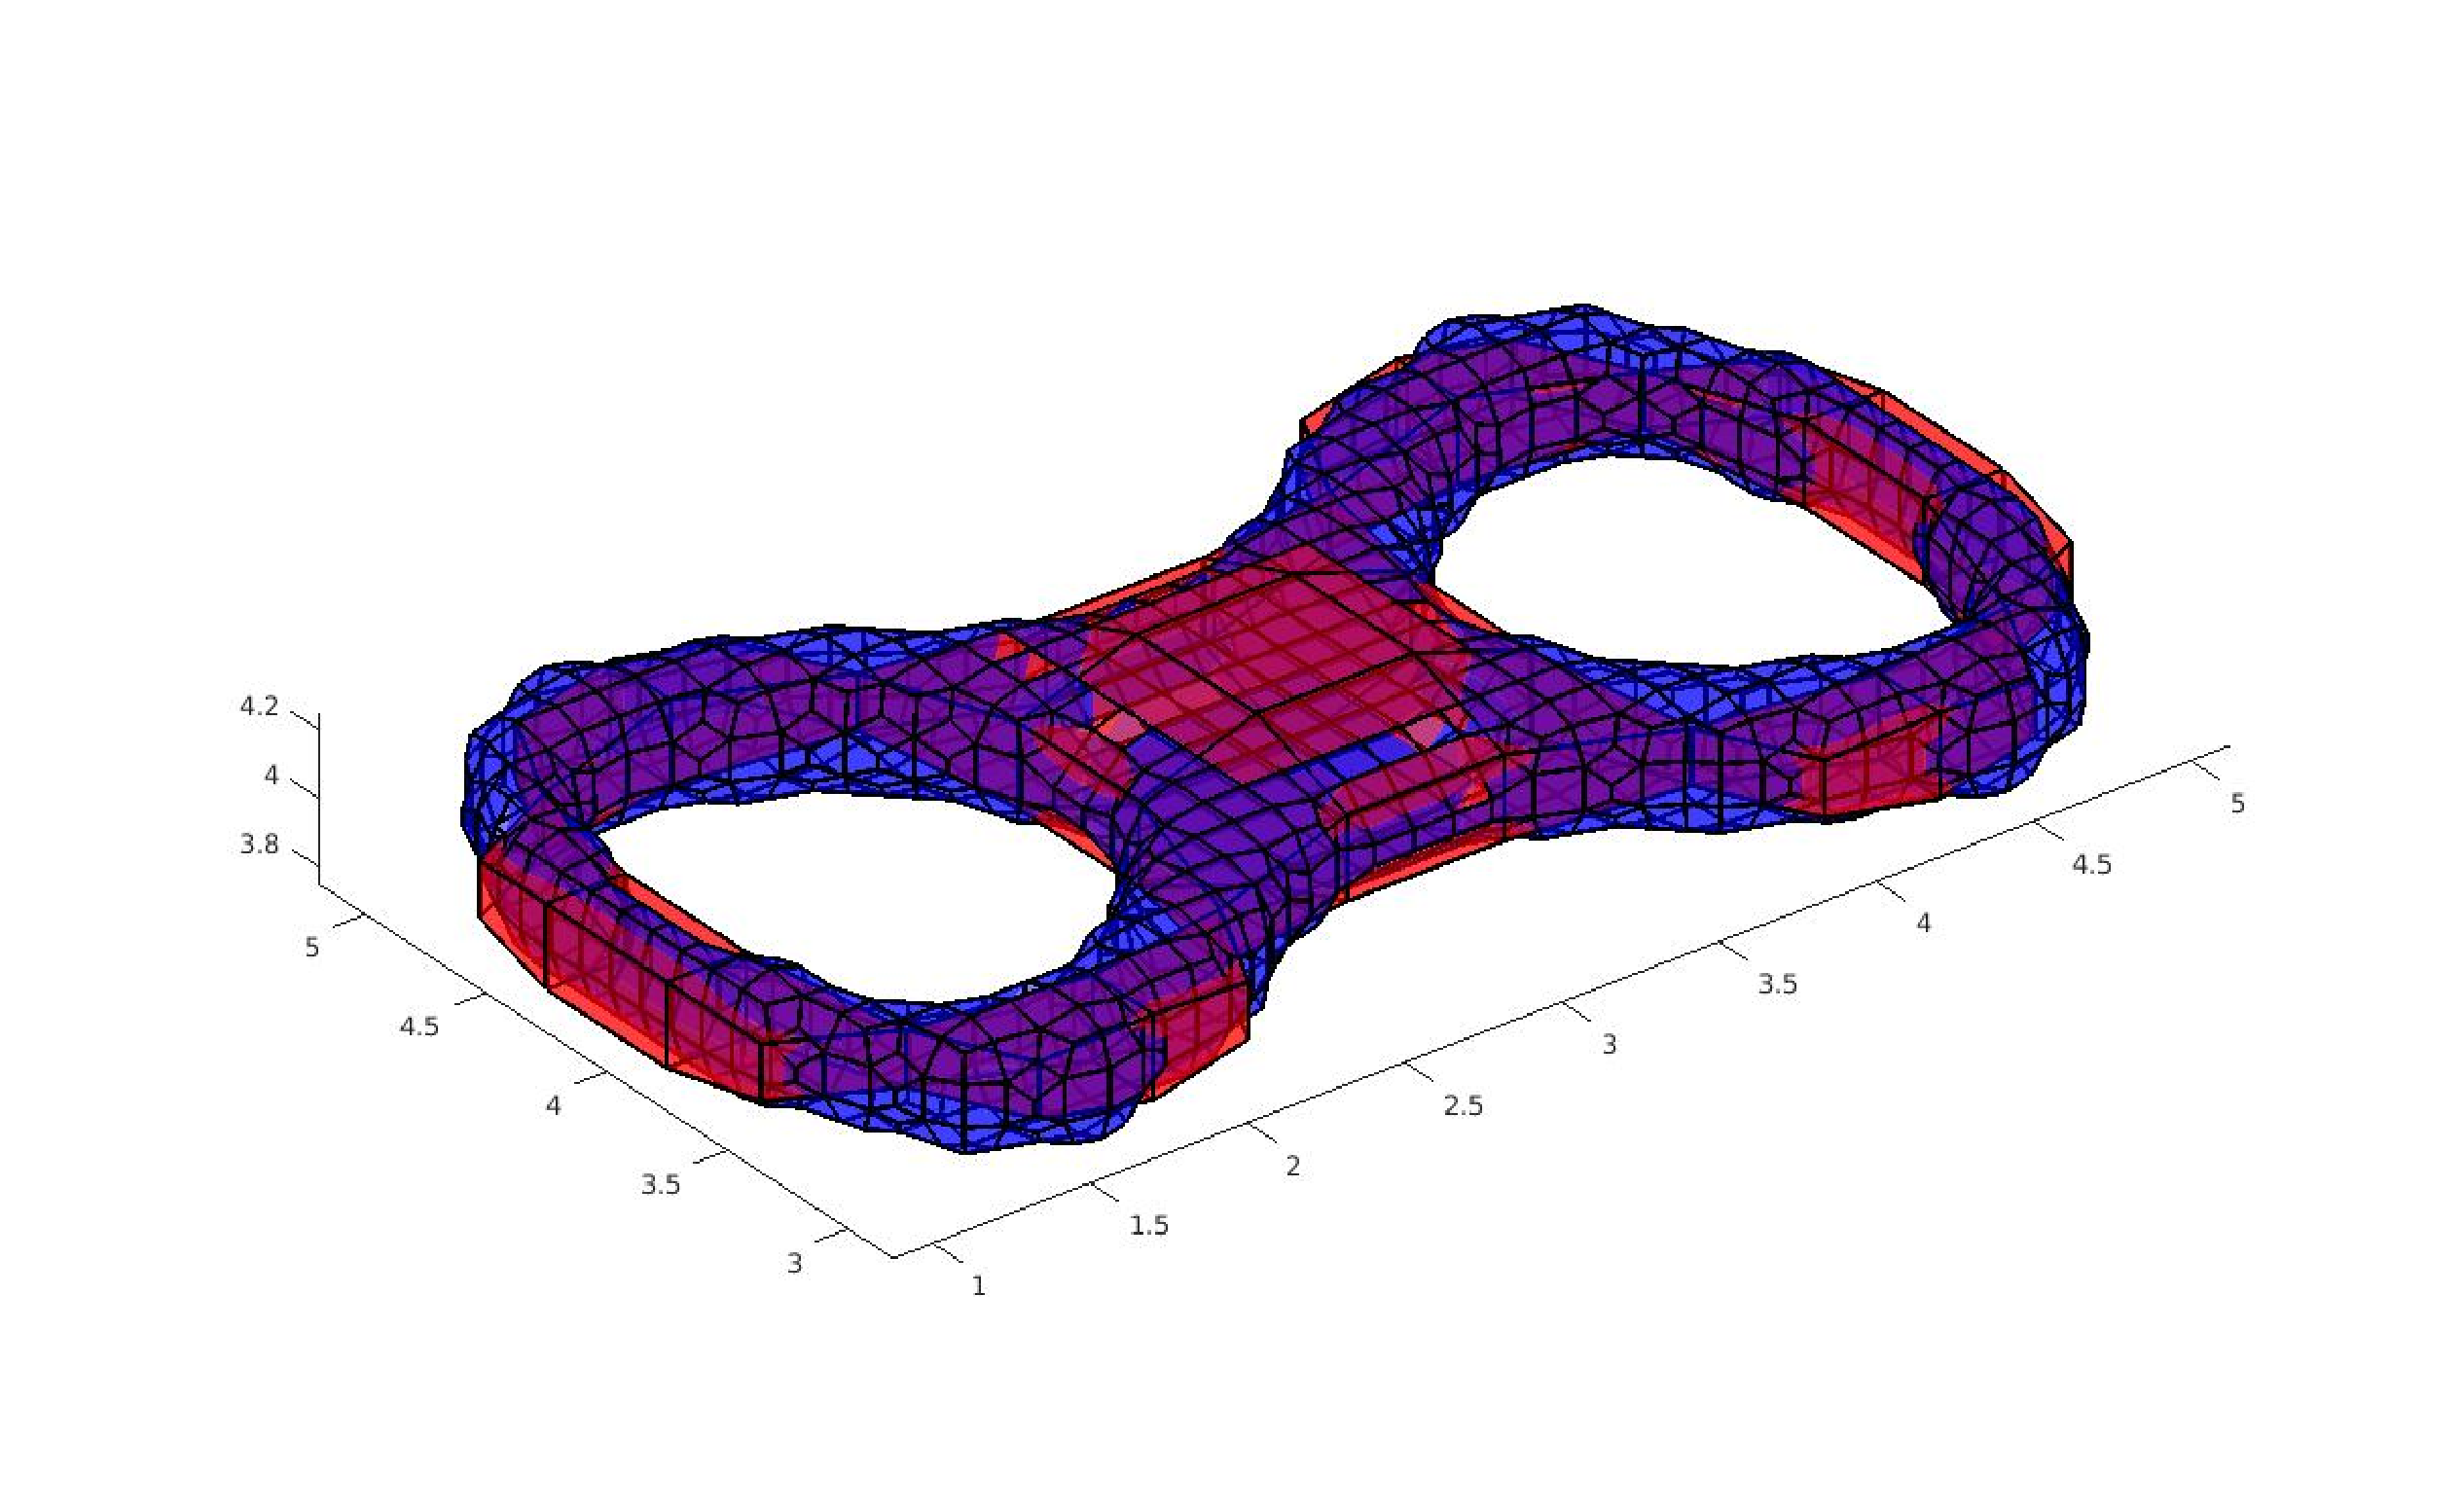
\includegraphics[scale=0.2]{Pictures/DC/doubleTorus.pdf}
	\end{figure}
	
\end{frame}

\begin{frame}

	\frametitle{Dual Contouring- Problems}
	
	\begin{itemize}
	\item  \textbf{Non-manifold edges} appear
	\item One edge can only belong to two quads for the surface to be closed
	\item Special treatments in the implementation to avoid them
	\end{itemize}
	\begin{figure}
	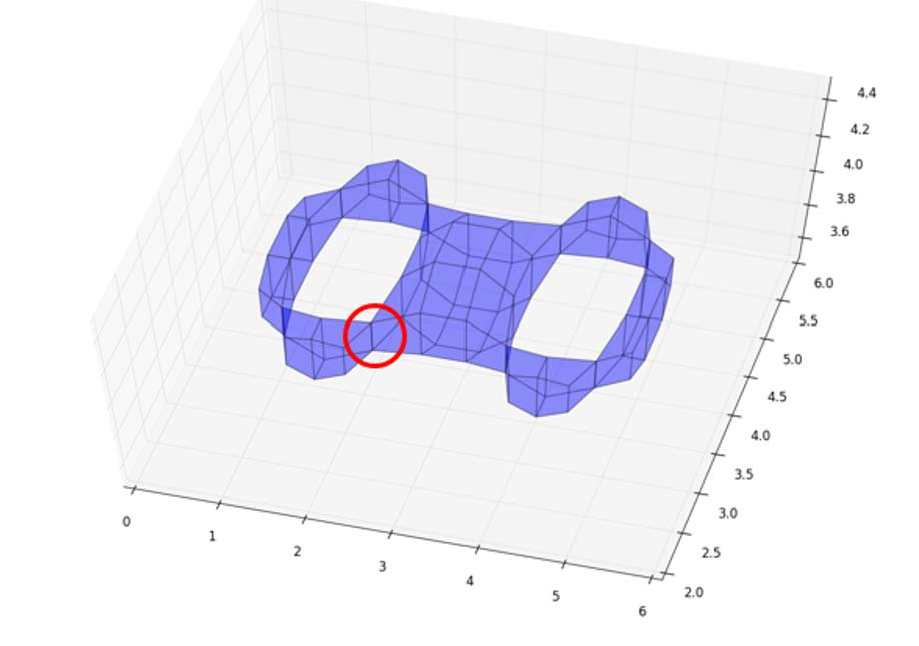
\includegraphics[scale=0.35]{Pictures/DC/manifolds.pdf}
	\end{figure}
	
\end{frame}

\begin{frame}

	\frametitle{Dual Contouring- Problems}
	
	\begin{itemize}
	\item  \textbf{Non-manifold edges} appear
	\item One edge can only belong to two quads for the surface to be closed
	\item Special treatments in the implementation to avoid them
	\end{itemize}
	\begin{figure}
	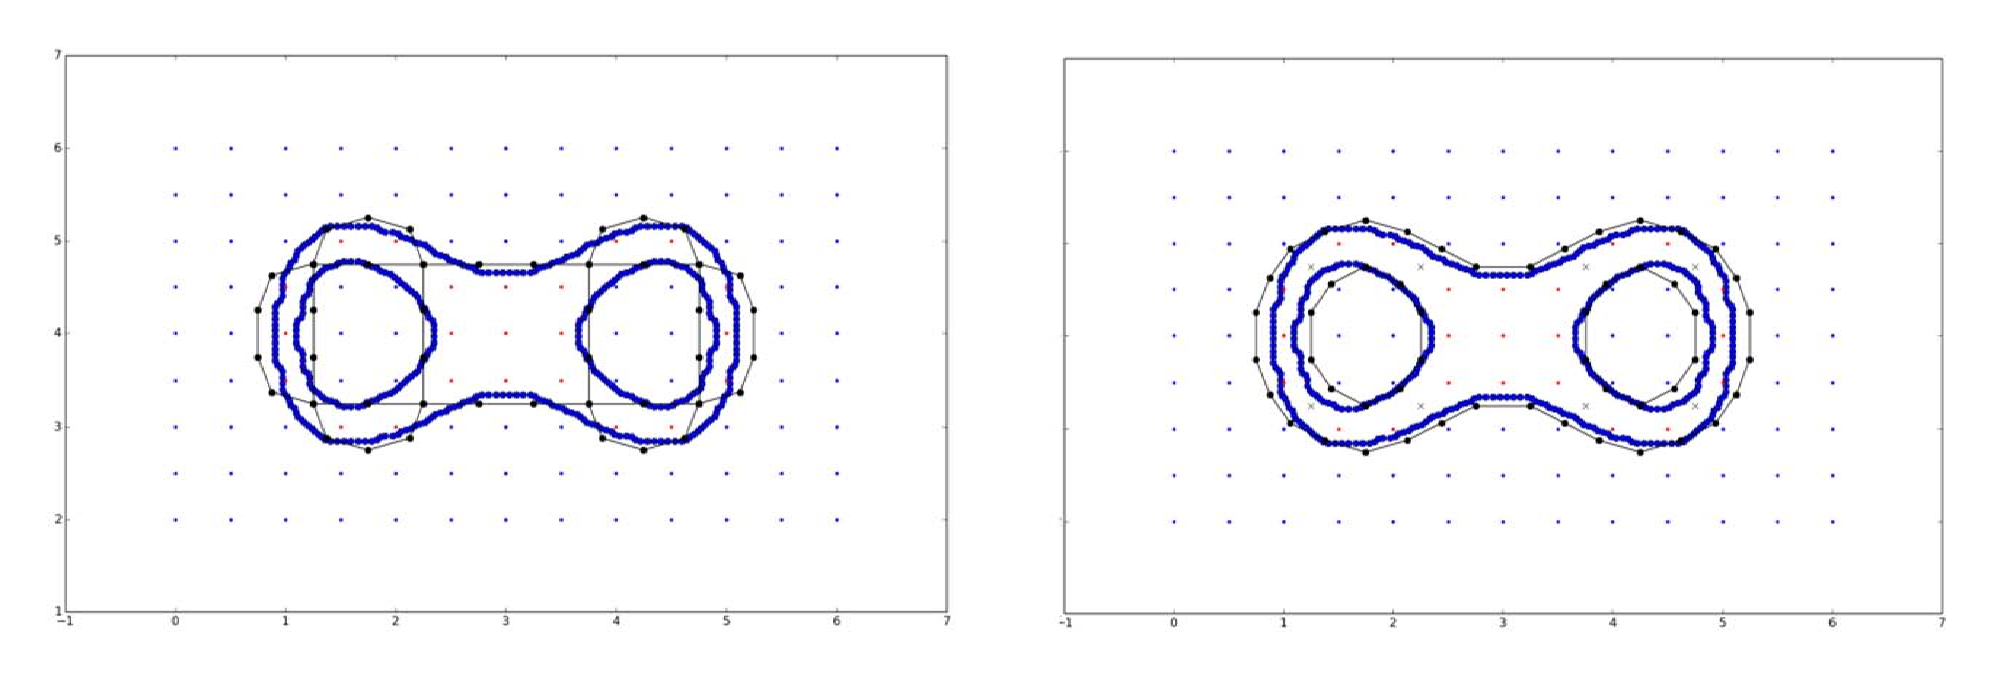
\includegraphics[scale=0.35]{Pictures/DC/DC_3.pdf}
	\end{figure}
	
\end{frame}

\begin{frame}

	\frametitle{Dual Contouring- Input}
	
	\begin{itemize}
	\item  Sixth step of the DRAFT pipeline- Interface between Topology Optimization and Surface Extraction
	\item Special implementation to use voxel data from Topy as input
	\end{itemize}
	\begin{figure}
	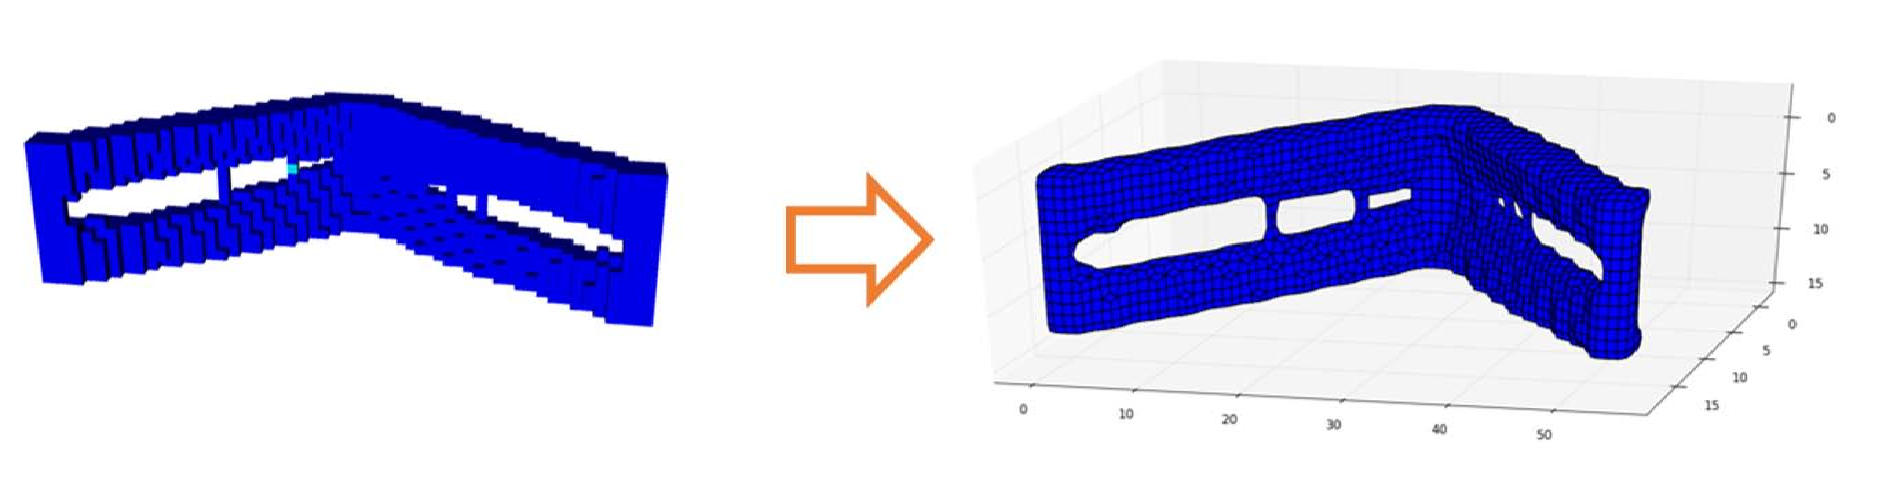
\includegraphics[scale=0.35]{Pictures/DC/cantilever.pdf}
	\end{figure}
	
\end{frame}

\begin{frame}

	\frametitle{Demo}
	

\end{frame}

\subsection{Projection and Parametrization}

\begin{frame}

	\frametitle{Projection and Parametrization}
	
	\begin{itemize}
	\item Points from finer grid are projected to quads of the coarser grid 
	\item Parameters \textit{u} and \textit{v} are found for each quad
	\item This information is needed for the algorithms in the last part of the pipeline
	\end{itemize}
	\begin{figure}
	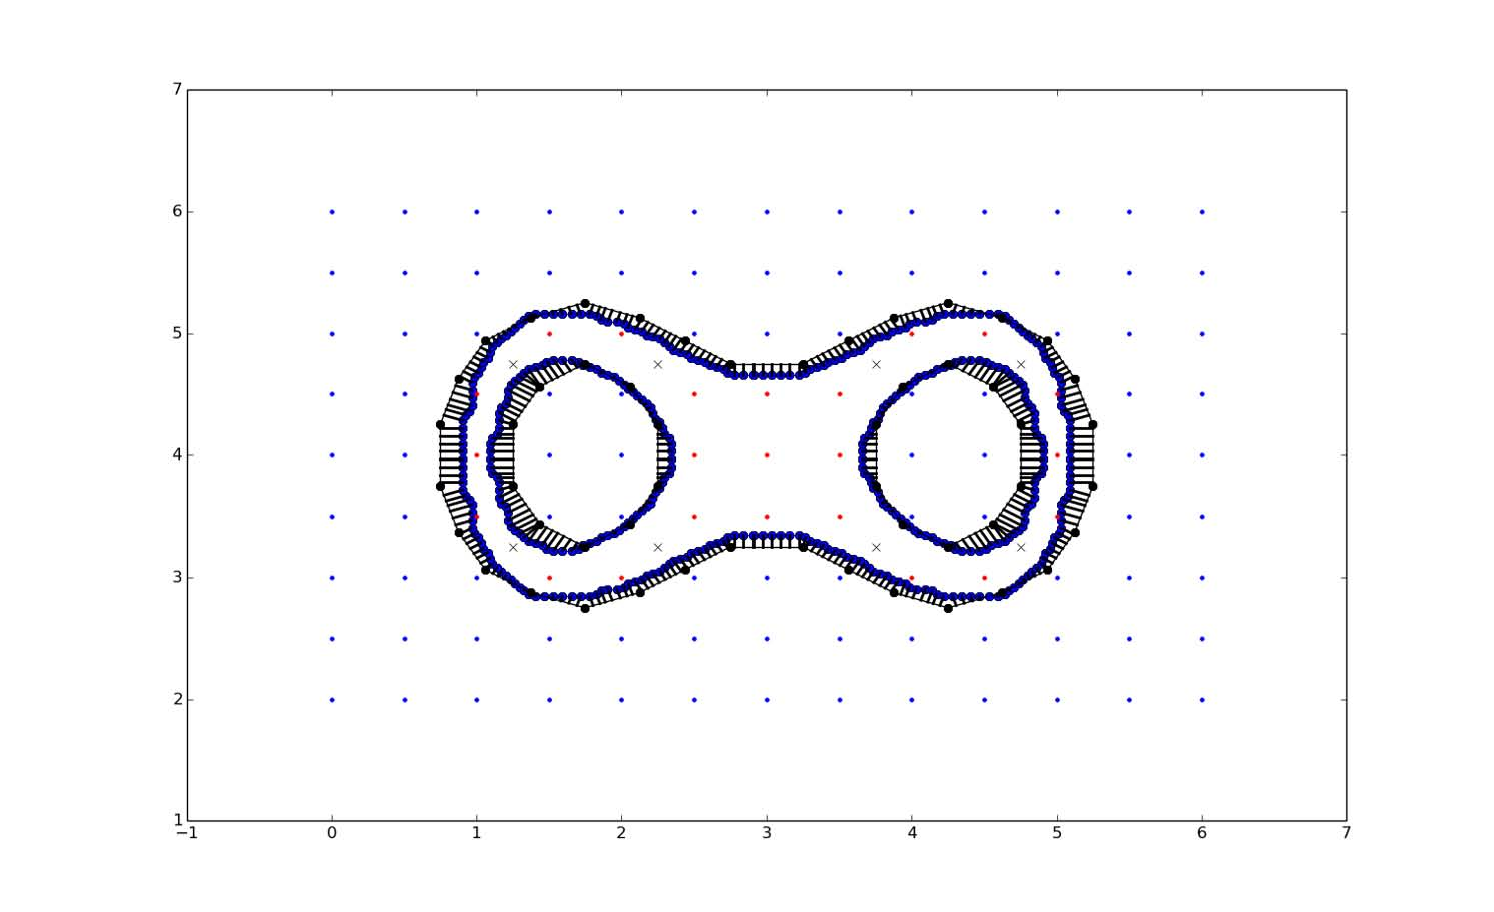
\includegraphics[scale=0.35]{Pictures/DC/DC_2.pdf}
	\end{figure}
	
\end{frame}





